\color{red}
\subsection{Enabling Side-Channel Aware Hardware Development}
While analysis of \textit{software} can be done using symbolic execution of the
software alongside a model of the hardware, symbolic execution is not a useful
tool for hardware designers attempting to determine if there exists
\textit{any} program which can leak information via a side-channel (i.e.,
symbolic execution cannot be used to determine if side-channel mitigation
techniques are adequate for \textit{all} possible programs).  This is because
symbolic execution considers all possible executions of a single program, not
all possible executions of all possible programs. In order to address this
shortcoming, we have developed a hardware model checking framework which
analyzes net switching behavior for arbitrary programs~\cite{bleier21}. This
was originally designed to generate microprocessors optimized to certain ISA
subsets.  Fig.~\ref{fig:pdat} shows an overview of this process, which we
call Property Driven Automatic Transformation (PDAT).
The inputs to PDAT are the microprocessor's
netlist, and two collections of properties.  The first, the `Property Library',
is a collection of properties for each type of gate in the netlist.  These
properties are used to capture gate switching activities.
The final input, the environmental restrictions, are properties describing
the possible inputs to the microprocessor (including all possible programs
and program data).  The environmental restrictions are used to ensure that
the model checkers only consider valid or legal programs and inputs, rather
than arbitrary programs and inputs.

\begin{wrapfigure}{l}{0.6\linewidth}
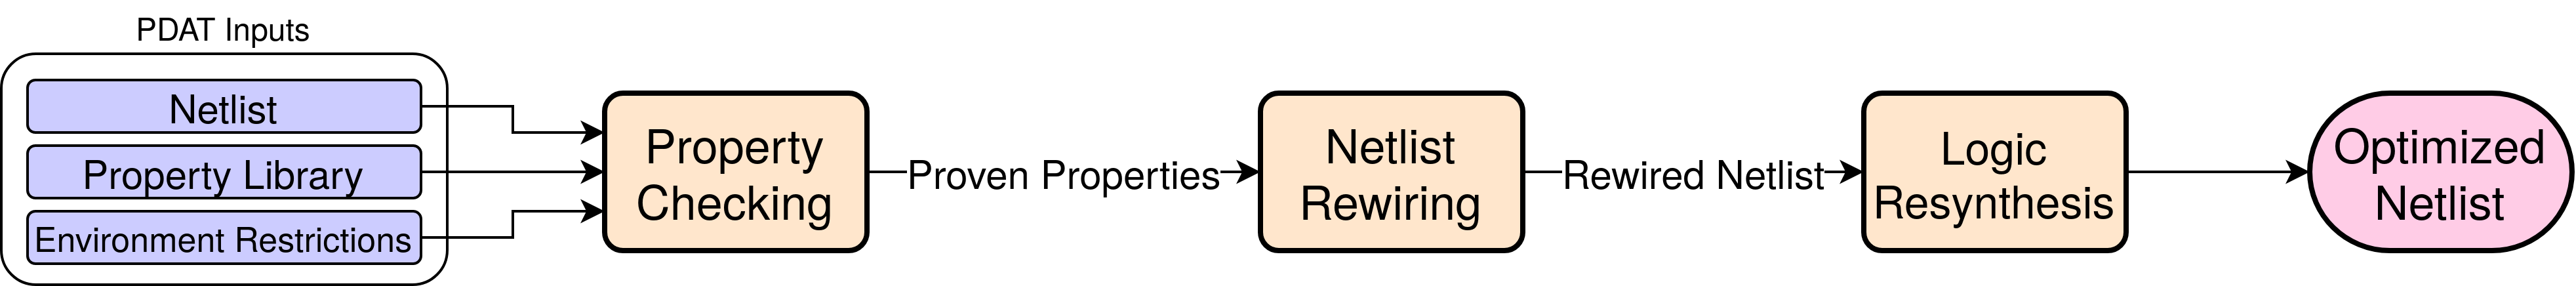
\includegraphics[width=\linewidth]{./figure/PDAT.png}
\caption{\small
    Model checking is used to identify gate switching behavior, and modify
    hardware appropriately.
}
\label{fig:pdat}
\end{wrapfigure}

Using model checking, in conjunction with microarchitectural hardware models,
designers can determine whether their design is resilient to EM side channel
leakage.  Since model checking provides witnesses to its proofs, it can
identify sequences of instruction/instruction classes and microarchitectural
events which lead to leakage of information via EM side-channel. PDAT, like the
symbolic execution framework which was originally intended to generate bespoke
microprocessors, may be repurposed to identify EM side-channel signatures.

\color{black}

